\documentclass[11pt,spanish,a4paper]{article}
% Versión 1.er cuat 2021 Víctor Bettachini < bettachini@df.uba.ar >

% Versión 1.er cuat 2021 Víctor Bettachini < bettachini@df.uba.ar >

\usepackage[T1]{fontenc}
\usepackage[utf8]{inputenc}

\usepackage[spanish, es-tabla]{babel}
\def\spanishoptions{argentina} % Was macht dass?
% \usepackage{babelbib}
% \selectbiblanguage{spanish}
% \addto\shorthandsspanish{\spanishdeactivate{~<>}}

\usepackage{graphicx}
\graphicspath{{./figuras/}}
% \usepackage{float}

\usepackage[arrowdel]{physics}
\newcommand{\pvec}[1]{\vec{#1}\mkern2mu\vphantom{#1}}
% \usepackage{units}
\usepackage[separate-uncertainty=true, multi-part-units=single, locale=FR]{siunitx}
\usepackage{isotope} % $\isotope[A][Z]{X}\to\isotope[A-4][Z-2]{Y}+\isotope[4][2]{\alpha}

\usepackage{tasks}
\usepackage[inline]{enumitem}
% \usepackage{enumerate}

\usepackage{hyperref}

% \usepackage{amsmath}
% \usepackage{amstext}
\usepackage{amssymb}

\usepackage{tikz}
\usepackage{tikz-dimline}
\usetikzlibrary{math}
\usetikzlibrary{arrows.meta}
% \usetikzlibrary{snakes}
% \usetikzlibrary{calc}
\usetikzlibrary{decorations.pathmorphing}
\usetikzlibrary{patterns}

\usepackage[hmargin=1cm,vmargin=1.6cm,nohead]{geometry}
% \voffset-3.5cm
% \hoffset-3cm
% \setlength{\textwidth}{17.5cm}
% \setlength{\textheight}{27cm}

\usepackage{lastpage}
\usepackage{fancyhdr}
\pagestyle{fancyplain}
\fancyhead{}
\fancyfoot{{\tiny \textcopyright DF, FCEyN, UBA}}
\fancyfoot[C]{ {\tiny Actualizado al \today} }
\fancyfoot[RO, LE]{Pág. \thepage/\pageref{LastPage}}
\renewcommand{\headrulewidth}{0pt}
\renewcommand{\footrulewidth}{0pt}


\begin{document}
\begin{center}
\textbf{Física 2} (Físicos) \hfill \textcopyright {\tt DF, FCEyN, UBA}\\
\textsc{\LARGE Condiciones iniciales de sistemas contínuos}
\end{center}

Los ejercicios con (*) son opcionales.

\begin{enumerate}

\subsection*{Evolución temporal de condiciones iniciales}

\item Los extremos fijos de una cuerda de longitud $L$ y densidad lineal $\mu_0$ la someten a una tensión $T_0$.
\begin{enumerate}
	\item Escriba la expresión más general posible para un modo normal en dicha cuerda y diga cuál es la velocidad de propagación de las ondas en ella.
	\item Determine con las condiciones de contorno los números de onda $k_p$, frecuencias y fases.
	Con esto, escriba la expresión general para una perturbación arbitraria $\psi(x,t)$.
	\item Obtenga $\psi(x,t)$ para el caso que parte del reposo con
	$
	\psi(x,0) = \sen{\left( \frac{3\pi x}{2L} \right)} \cos( \frac{\pi x}{2L} ).
	$
\end{enumerate}


\item Una cuerda de longitud $L$, densidad de masa uniforme $\mu_{0}$ está sujeta en ambos extremos lo que la somete a una tensión $T_{0}$.
A $t=0$ la cuerda se suelta de modo que su forma está dada por la siguiente función
$$
\psi(x,0) = \sen{ \left(\frac{\pi x}{L} \right) } + \frac{1}{3} \sen{ \left( \frac{3\pi x}{L} \right) } + \frac{1}{5} \sen{ \left( \frac{5\pi x}{L} \right) },
$$
si se toma un sistema de coordenadas tiene $x=0$ en un extremo de la soga y $x = L$ en el otro. 
%\begin{enumerate}
%	\item Halle $\psi(x,t)$.
%	\item 
	Si notamos la frecuencia fundamental como $\omega_{1}$, grafique $\psi(x,t)$ en $\omega_1 t = 0,\,\pi/5,\,\pi/3$ y $\pi/2$.
	¿Qué simetría tiene $\psi(x,t)$ en torno a $\omega_1 t = \pi/2$?
	¿Y de $\pi$?.
	¿Cómo sería $\psi(x,t)$ para $\omega_1 t = 2 \pi$?
%\end{enumerate}


\item Para una cuerda de longitud $L$, densidad lineal $\mu_{0}$ sometida a una tensión $T_0$ notamos su elongación transversal como $\psi(x,t)$.
\begin{enumerate}
	\item Escriba la expresión más general que representa un modo normal en
dicha cuerda, es decir, la expresión más general de una onda estacionaria.
	\item Sabiendo que la cuerda tiene un extremo libre y otro fijo, y que el
sistema de coordenadas con el que trabaja es tal que el extremo libre
está en $x=0$ y el extremo fijo está en $x=L$, imponga las condiciones
de contorno y determine las constantes pertinentes.
	\item Usando la relación de dispersión, obtenga las posibles frecuencias
temporales $\nu_{n}$. 
	\item Si $\psi(x,0)=0$ y $\dot{\psi}(x,0)=V_{0}\cos\left(\frac{3\pi}{2L}x\right)$, obtenga amplitud y fase de cada modo y luego $\psi(x,t)$.
\end{enumerate}


\item (*) Una cuerda de longitud $L$ sujeta en ambos extremos y sometida a una tensión $T_{0}$ consta de dos tramos de longitudes $L_1$ y $L_2$ y densidades de masa uniformes $\mu_1$ y $\mu_2$.
\begin{enumerate}
	\item Halle la expresión más general para un modo normal en dicha cuerda.
	Plantee las condiciones de contorno y halle las condiciones que deben cumplir los distintos parámetros.
	\item Halle los modos normales en este caso que $L_{1}=3L_{2}$ y $\mu_{2}=9\mu_{1}$. 
\end{enumerate}


\item (*) Una cuerda de densidad de masa uniforme $\mu$ y longitud $L$ está tensada $T_0$ entre extremos fijos.
Actúa una fuerza de amortiguamiento proporcional a su velocidad de oscilación.
Hallar la forma más general de $\psi(x,t)$.




\subsection*{Descomposición espectral de Condiciones iniciales}

\item
\begin{minipage}[t][2.3cm]{0.6\textwidth}
Una cuerda de densidad lineal de masa $\mu_{0}$ está sujeta en un extremo mientras el otro oscila libre manteniendo una tensión $T_{0}$.
En $t = 0$ se le impone la deformación dibujada (obvié el hecho de que eso es físicamente imposible sin modificar la homogeneidad de $\mu$).
La velocidad de propagación es \(v = \SI{80}{\metre\over\second} \).
\end{minipage}
\begin{minipage}[c][0.4cm][t]{0.34\textwidth}
	\begin{tikzpicture}
		\coordinate (quiebreInferior) at (1,0);
		\coordinate (quiebreSuperior) at (1,1);
		\coordinate (finalInferior) at (4,0);
		\coordinate (finalSuperior) at (4,1);
		\draw [-Latex] (0,0) -- (5,0) node [anchor=north] {\( x \)};	% eje x
		\draw [Latex-](0,2) node [anchor=west] {\( \psi(x,0) \)} -- (0,0) node [anchor=north] {\(0\)};	% eje y
		\draw [ultra thick] (0,0) -- (quiebreInferior);	% cuerda
		\draw [ultra thick] (quiebreSuperior) -- (finalSuperior);	% cuerda
		\draw [thin, dashed] (0,1) node [anchor=east] {\( \psi_0 \)} -- (quiebreSuperior);
		\draw [thin, dashed] (quiebreInferior) node [anchor=north] {\( L/4 \)} -- (quiebreSuperior);
		\draw [thin, dashed] (finalInferior) node [anchor=north] {\( L \)} -- (finalSuperior);
	\end{tikzpicture}
%	\includegraphics[width=\textwidth]{ej1-25}
\end{minipage}
\begin{enumerate}
	\item Halle $\psi(x,t)$ y grafíquelo para $\omega_1 t = 0,\,\pi$ y $2\pi$.
	\item Si tomara un sistema de coordenadas con el origen en el extremo libre de la cuerda, diga qué es lo que cambiaría.
	¿Es conveniente tal sistema?
\end{enumerate}





\item
\begin{minipage}[t][1.1cm]{0.6\textwidth}
¿Cuál \(L_1\) se maximiza la excitación del segundo modo?
¿Qué cambia musicalmente al cambiar \(L_1\)?
\end{minipage}
\begin{minipage}[c][1.5cm][t]{0.3\textwidth}
	\begin{tikzpicture}
		\draw [-Latex] (0,0) -- (5,0) node [anchor=north] {\( x \)};	% eje x
		\draw [Latex-](0,1) node [anchor=west] {\( \psi(x,0) \)} -- (0,0) node [anchor=north] {\(0\)};	% eje y
		\coordinate (L1) at (3,0.5);
		\coordinate (L1Inferior) at (3,0);
		\coordinate (L) at (4,0);
		\draw [ultra thick] (0,0) -- (L1) -- (L);	% cuerda
		\draw [thin, dashed] (0,0.5) node [anchor=east] {\( \psi_0 \)} -- (L1);
		\draw [thin, dashed] (L1Inferior) node [anchor=north] {\( L_1 \)} -- (L1);
		\draw [thin, dashed] (L) node [anchor=north] {\( L \)};
	\end{tikzpicture}
\end{minipage}



\item (*) Dada una cuerda de longitud $L$ y densidad de masa uniforme $\mu$, sometida a una tensión $T_{0}$ con ambos extremos fijos, demostrar que si $\psi(x,0)$ y $\dot{\psi}(x,0)$ son simétricas con respecto al centro de la cuerda, los modos con números de onda $k_{p}=2p\pi/L$ no se excitan.



\item
\begin{minipage}[t][2cm]{0.6\textwidth}
Un extremo de una cuerda de densidad lineal $\mu$ está fijo en tanto que está libre el que está a una distancia $L$.
Siempre se manteniendo una tensión $T_0$, en $t=0$ se la golpea sin deformarla pero imprimiéndole una velocidad $\dot{\psi}(x,0)$.
Halle $\psi(x,t>0)$.
\end{minipage}
\begin{minipage}[c][1cm][t]{0.49\textwidth}
	\begin{tikzpicture}
		\draw [-Latex] (0,0) -- (5,0) node [anchor=north] {\( x \)};	% eje x
		\draw [Latex-](0,1.5) node [anchor=west] {\( \dot{\psi}(x,0) \)} -- (0,0) node [anchor=north] {\(0\)};	% eje y
		\draw [ultra thick] (0,0) -- (2,0.5) -- (4,0.5);	% cuerda
		\draw [thin, dashed] (0,0.5) node [anchor=east] {\( \dot{\psi}_0 \)} -- (2,0.5);
		\draw [thin, dashed] (2,0) node [anchor=north] {\( L/2 \)} -- (2,0.5);
		\draw [thin, dashed] (4,0) node [anchor=north] {\( L \)} -- (4,0.5);
	\end{tikzpicture}
\end{minipage}




\subsection*{Descomposición espectral para gas en un tubo}

\item
\begin{minipage}[t][1.6cm]{0.65\textwidth}
(*) Un tubo contiene dos secciones de gas en reposo separadas por un tabique.
Antes de que se lo quite en $t=0$ de un lado la densidad era $\rho_{0}-\Delta$ y del otro $\rho_{0}+\Delta$ (considere $\Delta\ll\rho_{0}$).
Datos: $\rho_{0}$, $\Delta$, $L$, $v_\text{sonido}$.
\end{minipage}
\begin{minipage}[c][2cm][t]{0.3\textwidth}
	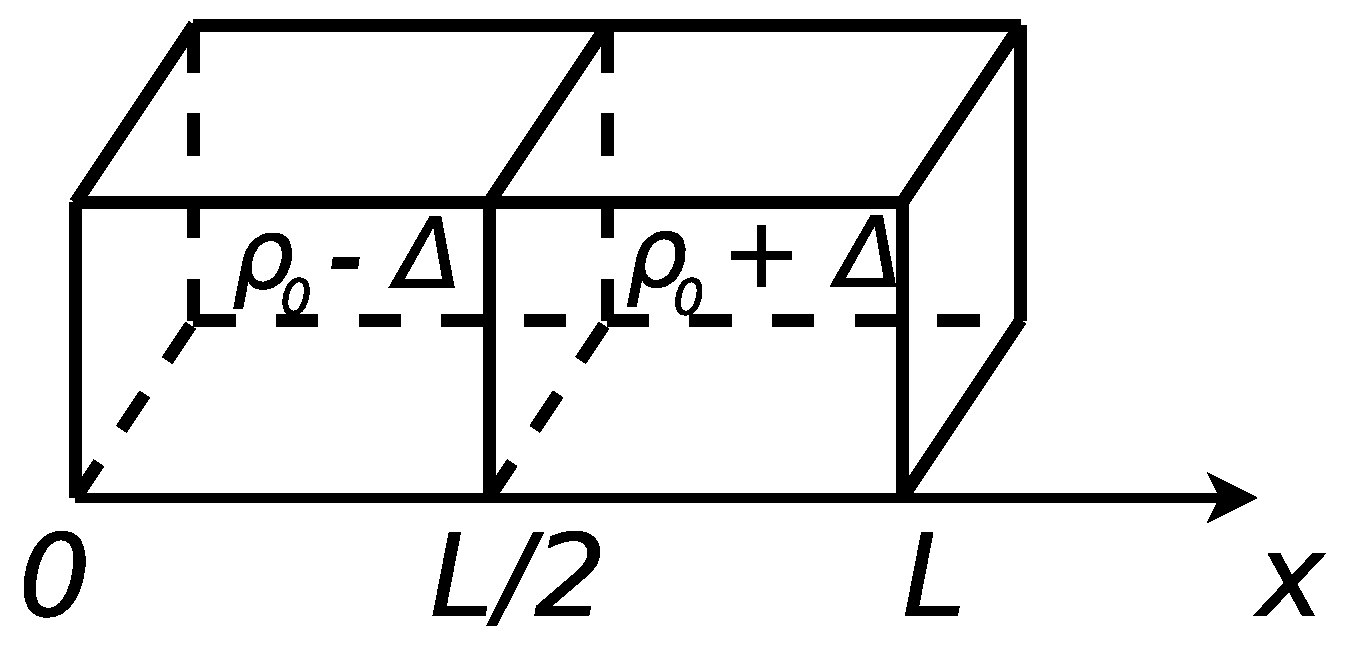
\includegraphics[width=\textwidth]{ej1-30}
\end{minipage}
\begin{enumerate}
	\item Imponga condiciones de contorno al desplazamiento de moléculas $\psi$.
	A partir de estas obtenga la expresión para un modo normal $\psi_{n}(x,t)$.
	¿Cuáles son las longitudes de onda permitidas?
	\item Halle $\psi(x,0)$ a partir de los datos sobre $\rho(x,0)$.
	\item Calcule $\psi(x,t)$ y $\rho(x,t)$.
\end{enumerate}


\item
\begin{minipage}[t][2cm]{0.65\textwidth}
(*) Un tabique divide un tubo dividido en dos regiones.
En la izquierda hay una presión constante $p = p_0 + \Delta p$ en tanto que en la derecha está a $p_0$ pues está abierta a la atmósfera.
A $t = 0$ se remueve el tabique.

Halle $\delta p(x,t)$, $\psi(x,t)$ y $\delta\rho(x,t)$ conociendo $p_0$, $\Delta p\ll p_0$, $L$, $v_\text{sonido}$ y que $\gamma= \frac{7}{5}$ para un gas diatómico.
\end{minipage}
\begin{minipage}[c][0.6cm][t]{0.3\textwidth}
	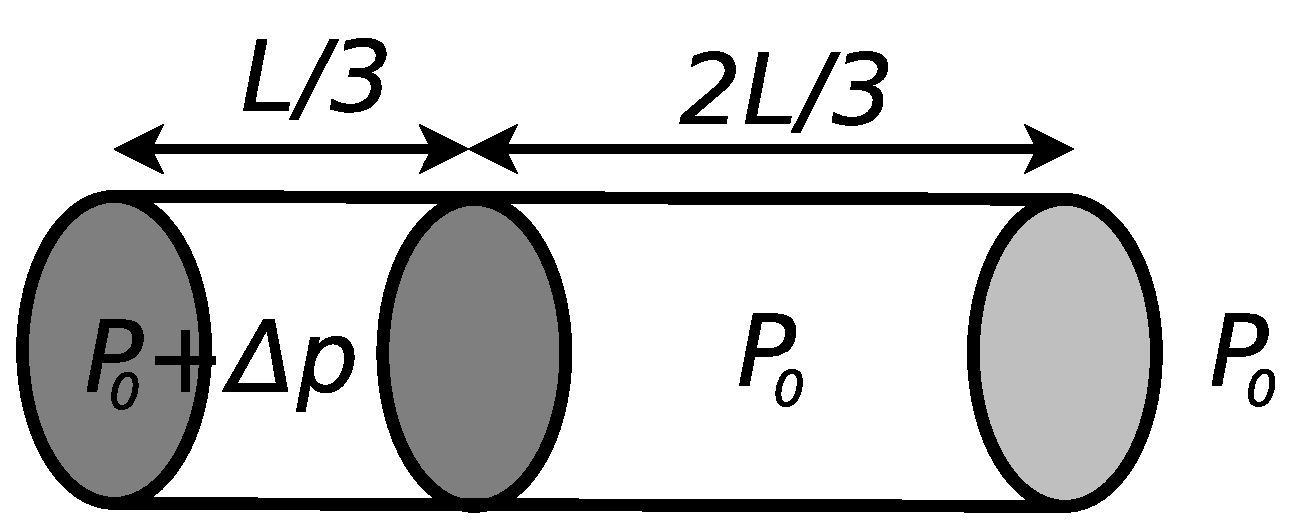
\includegraphics[width=\textwidth]{ej1-31}
\end{minipage}



gg
\end{enumerate}

\end{document}
